
%(BEGIN_QUESTION)
% Copyright 2010, Tony R. Kuphaldt, released under the Creative Commons Attribution License (v 1.0)
% This means you may do almost anything with this work of mine, so long as you give me proper credit

Work with your instructor to set up a test fixture to demonstrate reflected pulses on a transmission line.  For this experiment, you will need:

\begin{itemize}
\item{} Spool of multi-conductor cable (twisted-pair preferred)
\item{} Oscilloscope
\item{} Signal generator with square-wave output
\item{} Resistor (100 ohms)
\item{} Low-value potentiometer (adjustable to near 100 ohms with ease)
\item{} Ohmmeter
\end{itemize}

Connect these components together as shown:

$$\includegraphics[width=15.5cm]{i04410x01.eps}$$

With no potentiometer connected at the cable's far end, analyze the square-wave signal showing on the oscilloscope screen.  Start with low-frequency signals (e.g. 100 Hz) and then work upwards to higher and higher frequencies, until you see a ``step'' distortion appearing on the leading edge of each pulse.  Carefully note the width of the ``step'' distortion as you increase and decrease signal generator frequency -- does this width change with frequency?  Why or why not?  Measure the time-width of this step.

\vskip 10pt

After noting the waveform with an open-ended transmission line, connect a jumper wire to the cable end to act as a dead short, noting how this affects the waveform's shape.  Which part(s) of the waveform looks the same as the open-ended cable test?  Which part(s) of the waveform look different from the previous test?

\vskip 10pt

Finally, connect the potentiometer to the cable's end to function as a variable terminating resistor.  Note the appearance of the waveform as the potentiometer's value is increased and decreased.  Adjust the potentiometer until the square-wave signal appears undistorted, then disconnect the potentiometer and read its value with an ohmmeter -- this is the {\it characteristic impedance} value of the cable!

\vskip 10pt

Relate the measured width of the ``step'' distortion seen in both open-ended and shorted cable tests.  Mathematically relate this width to the length of the cable.

\underbar{file i04410}
%(END_QUESTION)





%(BEGIN_ANSWER)

The relationship between ``step'' distortion width and cable length is as follows:

$$t = {2x \over v}$$

\noindent
Where,

$t$ = Width of ``step'' in seconds

$x$ = Cable length in feet or meters

$v$ = Velocity of propagation in feet per second or meters per second

\vskip 10pt

%(END_ANSWER)





%(BEGIN_NOTES)

\vfil \eject

\noindent
{\bf Summary Quiz:}

Calculate the length of a cable with a velocity factor of 0.75 if the time delay between the incident and reflected pulses measured at the signal input end of the cable is 0.38 microseconds.  Recall that the speed of light in a vacuum is $3 \times 10^8$ meters per second.

\begin{itemize}
\item{} 42.75 meters 
\vskip 5pt 
\item{} 38.0 meters
\vskip 5pt 
\item{} 114 meters
\vskip 5pt 
\item{} 21.38 meters
\vskip 5pt 
\item{} 57.0 meters
\vskip 5pt 
\item{} 85.5 meters
\end{itemize}


%INDEX% Electronics review: characteristic impedance of transmission line
%INDEX% Electronics review: surge impedance of transmission line

%(END_NOTES)

